\begin{center}
    \textit{Heaven’s Light is Our Guide} \\
    \vspace{1cm}
    \Large{Rajshahi University of Engineering \& Technology} \\
    \vspace{1cm}
    
\includegraphics[width=3cm]{ruet-logo.png}\\
    \vspace{0.1cm}
    \Large{Department of Computer Science and Engineering} \\
    \vspace{1cm}
    \large{\textbf{Course no:} CSE 4204} \\
    \large{\textbf{Course Title:} Sessional Based on CSE 4203} \\
    \large{\textbf{Experiment no:} 3}\\
    \large{\textbf{Name of the experiment:}} \\
    \large{Design and implementation of Multi-layer
    Neural Networks algorithm (i.e., Back-propagation learning neural
    networks algorithm).} \\
    \vspace{1cm}
\end{center}
\thispagestyle{empty}
\Large{\textbf{Submitted by}}\\
Partho Kumar Rajvor \\
Roll: 1803119 \\
Section: B \\
Department of Computer Science and Engineering\\
Rajshahi University of Engineering and Technology\\\\
\Large{\textbf{Submitted to}}\\
Rizoan Toufiq \\
Assistant Professor \\
Department of Computer Science and Engineering \\
Rajshahi University of Engineering and Technology
\tableofcontents

\setcounter{chapter}{2}
\chapter{Design and implementation of Multi-layer
Neural Networks algorithm}
\section{Introduction}
Multilater perceptron (MLP) is a feedforward artificial neural network that generates a set of outputs from a set of inputs. An MLP is characterized by several layers of input nodes connected as a directed graph between the input and output layers. MLP uses backpropogation for training the network. MLP is a deep learning method.\\\\
MLP requires labeled dataset for training. MLP is used for classification and regression problems. MLP is also used for time series prediction, image recognition and voice recognition.\\

\section{About the dataset}
In this lab, we will be using the same dataset as we used in the previous lab.\\
\subsection{Foreword}
We will be using the following libraries in this lab:
\begin{itemize}
    \item \textit{pandas} for loading and preprocessing the dataset.
    \item \textit{scikit-learn} for splitting the dataset into training and test sets and measuring performance metrics of the model.
\end{itemize}
\subsection{Preprocessing the dataset}
To ease the process of working with the dataset, we will specifically preprocess the \textit{disagnosis} column of the dataset. We will replace the values \textit{M} and \textit{B} with 1 and 0 respectively. This will help us to work with the dataset more easily.
\begin{lstlisting}[language=Python]
    df['diagnosis'] = df['diagnosis']
                        .replace('M', 1)
    df['diagnosis'] = df['diagnosis']
                        .replace('B', 0)
\end{lstlisting}
\subsection{Selecting the features and the output}
We will be using the first 30 columns of the dataset as the features and the last column as the output. We will use the following code snippet to select the features and the output:
\begin{lstlisting}[language=Python]
    x = df.iloc[:, 2:32]
    y = df.iloc[:, 1]
\end{lstlisting}
\section{Implementing the MLP algorithm}
\subsection{Algotihm of the MLP}
\begin{enumerate}
    \item Initialize the weights and thresholds with random values.
    Set all the weights and thresholds to some small random values.
    \item Present input and desired output patterns.
    Present input $X_p$ = $x_0$, $x_1$, $x_2$, ..., $x_n$ and target output $t_p$ = $t_0$, $t_1$, $t_2$, ..., $t_m-1$ where $x_0$ = 1 and $w_0$ is the threshold.
    \item Calculate actual output.
    Each layer compute its actual output using the following formula:\\
    $y_{pj}$ = $f$[$\sum_{i=0}^{n-1} w_{i}x_{i}$]\\
    and passes it to the next layer.
    \item Adapt weights:\\
    Start from the last layer and move backward.\\
    For the last layer, the error is calculated as:\\
    $\delta_{pj}$ = $y_{pj}(1-y_{pj})(t_{pj}-y_{pj})$\\\\
    For the hidden layers, the error is calculated as:\\
    $\delta_{pj}$ = $y_{pj}(1-y_{pj})\sum_{k=0}^{m-1} w_{kj}\delta_{pk}$\\\\
    The weights are updated using the following formula:\\
    $w_{ij}(t+1)$ = $w_{ij}(t)$ + $\eta\delta_{pj}x_{ij}$\\
    where $\eta$ is the learning rate.\\\\
\end{enumerate}
\subsection{Necessary imports}
\begin{minted}{Python}
import numpy as np
import pandas as pd
from sklearn.model_selection import train_test_split
from sklearn.metrics import confusion_matrix, 
                            accuracy_score, 
                            f1_score
\end{minted}
\subsection{Implementing the algorithm}
\begin{minted}{python}
    class MLP:
    def __init__(self, 
        num_inputs, 
        hidden_layers=[10, 10], 
        num_outputs=2, 
        epochs=100, 
        learning_rate=0.1):
        # using default hidden layers of 10, 10
        self.num_inputs = num_inputs
        self.hidden_layers = hidden_layers
        self.num_outputs = num_outputs
        self.epochs = epochs
        self.learning_rate = learning_rate

        layers = [num_inputs] + 
                hidden_layers + 
                [num_outputs]

        # initiate random weights 
        weights = []
        for i in range(len(layers) - 1):
            w = np.random.rand(layers[i], 
                        layers[i + 1])
            weights.append(w)
        self.weights = weights


        # init derivatives
        self.derivatives = [np.zeros(w.shape) 
                            for w in self.weights]

        # init activations  
        self.activations = [np.zeros(i) 
                            for i in layers]


    def forward_propagate(self, x):
        # save input into activations
        activations = x 
        self.activations[0] = activations

        for idx, w in enumerate(self.weights):
            net_inputs = np.dot(activations, w)
            activations = self._sigmoid(net_inputs)
            self.activations[idx + 1] = activations

        return activations


    def back_propagate(self, error):
        for i in reversed(
                    range(
                        len(self.derivatives)
                        )
                    ):
            activations = self.activations[i+1]
            delta = error * self._sigmoid_derivative(
                            activations)
            delta_re = delta
                        .reshape(delta.shape[0], -1)
                        .T
            current_activations = self.activations[i]
            current_activations = current_activations
                                .reshape
                                (
                                    current_activations
                                    .shape[0],
                                -1)
            self.derivatives[i] = np.dot(
                            current_activations,
                            delta_re)
            error = np.dot(delta, self.weights[i].T)


    def train(self, inputs, targets):
        for i in range(self.epochs):
            sum_errors = 0
            for j, input in enumerate(inputs):
                target = targets[j]
                output = self.forward_propagate(input)
                error = target - output
                self.back_propagate(error)
                self.gradient_descent()
                sum_errors += self.
                    _calc_error(target, output)
            print("Error: {} at epoch {}"
                    .format(
                    sum_errors / len(inputs), i+1)
                    )
        print("Training completed")

    def gradient_descent(self):
        # update the weights by 
        # stepping down the gradient
        for i in range(len(self.weights)):
            weights = self.weights[i]
            derivatives = self.derivatives[i]
            weights += derivatives * self.learning_rate 


    def _sigmoid(self, x):
        y = 1.0 / (1 + np.exp(-x))
        return y


    def _sigmoid_derivative(self, x):
        return x * (1.0 - x)

    def _calc_error(self, target, output):
        return np.average((target - output) ** 2)
    
    def predict(self, X):
        y_pred = []
        for i in range(len(X)):
            y_pred.append(self.forward_propagate(X[i]))
        return np.array(y_pred).round()
\end{minted}
\subsection{Splitting the dataset into training and test sets}
We will be using the \textit{scikit-learn} library to split the dataset into training and test sets. We will use the following code snippet to split the dataset into training and test sets:
\begin{lstlisting}[language=Python]
    X_train, X_test, y_train, y_test = 
    train_test_split(X, y, test_size=0.2)
    X_train = np.array(X_train)
    X_test = np.array(X_test)
    y_train = np.array(y_train)
    y_test = np.array(y_test)
\end{lstlisting}
\section{Training the model and evaluating the performance}
\subsection{Training the model}
Let us use two hidden layers with 30 neurons each.
\begin{lstlisting}[language=Python]
mlp = MLP(num_inputs=len(X_train[0]),
         hidden_layers=[X_train[0], X_train[0]], 
         num_outputs=1, 
         epochs=10000, 
         learning_rate=0.1)
mlp.train(X_train, y_train)
y_pred = mlp.predict(X_test)
\end{lstlisting}
\subsection{Accuracy of the model}
We will use the following code snippet to calculate the accuracy of the model:
\begin{lstlisting}[language=Python]
acc = accuracy_score(y_test, y_pred)
print(f'Accuracy: {acc}')
cm = confusion_matrix(y_test, y_pred)
print(f'Confusion Matrix:\n{cm}')
f1 = f1_score(y_test, y_pred)
print(f'F1 Score: {f1}')
\end{lstlisting}
\subsection{Output}
Accuracy: 0.9385964912280702\\
Confusion Matrix:
$$
\begin{bmatrix}
71 & 2 \\
8 & 33
\end{bmatrix}
$$\\
F1 Score: 0.9113924050632912

\section{Visualization of the results}
\subsection{Scatter plot using testing input and predicted output}
We will be using two features to plot the scatter plot.
\begin{lstlisting}[language=Python]
plt.scatter(X_test[:, 0], X_test[:, 1], c=pred)
plt.title("Predicted")
plt.show()
\end{lstlisting}
\begin{figure}[ht]
    \centering
    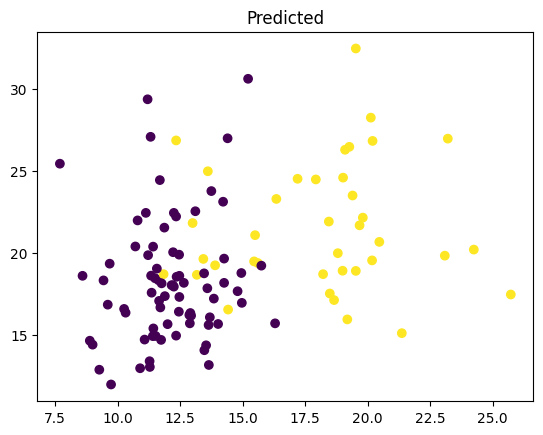
\includegraphics[width=10cm]{ch/figures/scatter4.png}
    \caption{Scatter plot using testing input and predicted output}
    \label{fig:scatter4}
\end{figure}
\subsection{Scatter plot using testing input and desired output}
We will be using two features to plot the scatter plot.
\begin{lstlisting}[language=Python]
plt.scatter(X_test[:, 0], X_test[:, 1], c=y_test)
plt.title("Desired")
plt.show()
\end{lstlisting}
\begin{figure}[ht]
    \centering
    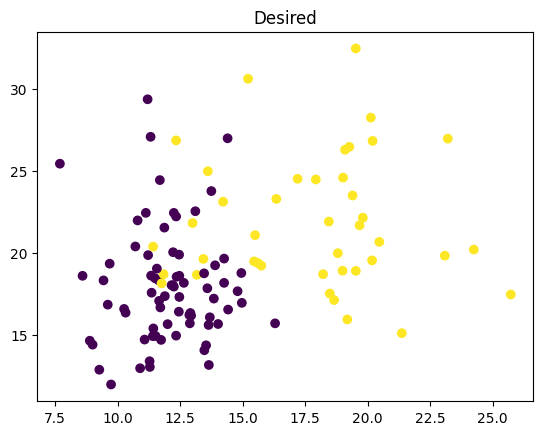
\includegraphics[width=10cm]{ch/figures/scatter5.png}
    \caption{Scatter plot using testing input and desired output}
    \label{fig:scatter5}
\end{figure}
\break
\subsection{Confusion Matrix}
\begin{figure}[ht]
    \centering
    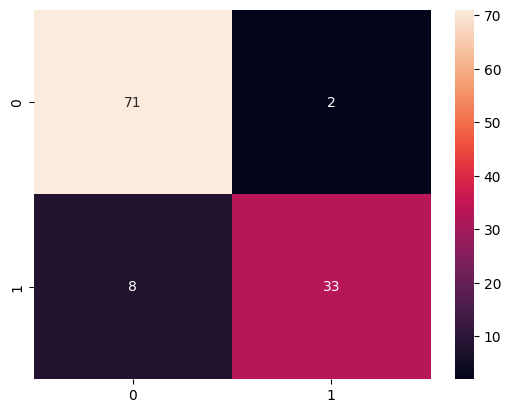
\includegraphics[width=8cm]{ch/figures/cm4.png}
    \caption{Confusion Matrix}
    \label{fig:loss}
\end{figure}
\newpage
\subsection{Visualizing Error vs Iteration}
Here we are only showing error upto 1000 iterations.
\begin{figure}[ht]
    \centering
    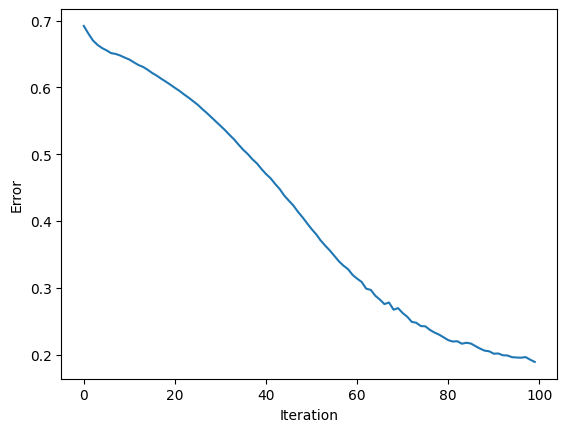
\includegraphics[width=8cm]{ch/figures/loss.png}
    \caption{Error vs Iteration}
    \label{fig:loss}
\end{figure}
\newpage
\section{Solving XOR problem using MLP}
\subsection{Training the model}
Let us use two hidden layers with 5 neurons each.
\begin{lstlisting}[language=Python]
X = np.array([[0, 0], [0, 1], [1, 0], [1, 1]])
y = np.array([0, 1, 1, 0])
mlp = MLP(num_inputs=2, 
hidden_layers=[5, 5], 
num_outputs=1, 
epochs=20000, 
learning_rate=0.1)
mlp.train(X, y)
pred = mlp.predict(X)
print("pred: ", pred)
acc = accuracy_score(y, y_pred)
print(f'Accuracy: {acc}')
\end{lstlisting}
\subsection{Output}
pred:  [[0.]
 [1.]
 [1.]
 [0.]]
\subsection{Accuracy of the model}
Accuracy score: 1.0


\section{Conclusion}





